\documentclass[twoside]{book}

% Packages required by doxygen
\usepackage{fixltx2e}
\usepackage{calc}
\usepackage{doxygen}
\usepackage[export]{adjustbox} % also loads graphicx
\usepackage{graphicx}
\usepackage[utf8]{inputenc}
\usepackage{makeidx}
\usepackage{multicol}
\usepackage{multirow}
\PassOptionsToPackage{warn}{textcomp}
\usepackage{textcomp}
\usepackage[nointegrals]{wasysym}
\usepackage[table]{xcolor}

% Font selection
\usepackage[T1]{fontenc}
\usepackage[scaled=.90]{helvet}
\usepackage{courier}
\usepackage{amssymb}
\usepackage{sectsty}
\renewcommand{\familydefault}{\sfdefault}
\allsectionsfont{%
  \fontseries{bc}\selectfont%
  \color{darkgray}%
}
\renewcommand{\DoxyLabelFont}{%
  \fontseries{bc}\selectfont%
  \color{darkgray}%
}
\newcommand{\+}{\discretionary{\mbox{\scriptsize$\hookleftarrow$}}{}{}}

% Page & text layout
\usepackage{geometry}
\geometry{%
  a4paper,%
  top=2.5cm,%
  bottom=2.5cm,%
  left=2.5cm,%
  right=2.5cm%
}
\tolerance=750
\hfuzz=15pt
\hbadness=750
\setlength{\emergencystretch}{15pt}
\setlength{\parindent}{0cm}
\setlength{\parskip}{3ex plus 2ex minus 2ex}
\makeatletter
\renewcommand{\paragraph}{%
  \@startsection{paragraph}{4}{0ex}{-1.0ex}{1.0ex}{%
    \normalfont\normalsize\bfseries\SS@parafont%
  }%
}
\renewcommand{\subparagraph}{%
  \@startsection{subparagraph}{5}{0ex}{-1.0ex}{1.0ex}{%
    \normalfont\normalsize\bfseries\SS@subparafont%
  }%
}
\makeatother

% Headers & footers
\usepackage{fancyhdr}
\pagestyle{fancyplain}
\fancyhead[LE]{\fancyplain{}{\bfseries\thepage}}
\fancyhead[CE]{\fancyplain{}{}}
\fancyhead[RE]{\fancyplain{}{\bfseries\leftmark}}
\fancyhead[LO]{\fancyplain{}{\bfseries\rightmark}}
\fancyhead[CO]{\fancyplain{}{}}
\fancyhead[RO]{\fancyplain{}{\bfseries\thepage}}
\fancyfoot[LE]{\fancyplain{}{}}
\fancyfoot[CE]{\fancyplain{}{}}
\fancyfoot[RE]{\fancyplain{}{\bfseries\scriptsize Generated by Doxygen }}
\fancyfoot[LO]{\fancyplain{}{\bfseries\scriptsize Generated by Doxygen }}
\fancyfoot[CO]{\fancyplain{}{}}
\fancyfoot[RO]{\fancyplain{}{}}
\renewcommand{\footrulewidth}{0.4pt}
\renewcommand{\chaptermark}[1]{%
  \markboth{#1}{}%
}
\renewcommand{\sectionmark}[1]{%
  \markright{\thesection\ #1}%
}

% Indices & bibliography
\usepackage{natbib}
\usepackage[titles]{tocloft}
\setcounter{tocdepth}{3}
\setcounter{secnumdepth}{5}
\makeindex

% Hyperlinks (required, but should be loaded last)
\usepackage{ifpdf}
\ifpdf
  \usepackage[pdftex,pagebackref=true]{hyperref}
\else
  \usepackage[ps2pdf,pagebackref=true]{hyperref}
\fi
\hypersetup{%
  colorlinks=true,%
  linkcolor=blue,%
  citecolor=blue,%
  unicode%
}

% Custom commands
\newcommand{\clearemptydoublepage}{%
  \newpage{\pagestyle{empty}\cleardoublepage}%
}

\usepackage{caption}
\captionsetup{labelsep=space,justification=centering,font={bf},singlelinecheck=off,skip=4pt,position=top}

%===== C O N T E N T S =====

\begin{document}

% Titlepage & ToC
\hypersetup{pageanchor=false,
             bookmarksnumbered=true,
             pdfencoding=unicode
            }
\pagenumbering{alph}
\begin{titlepage}
\vspace*{7cm}
\begin{center}%
{\Large C\+S\+E-\/498-\/011-\/\+S\+P21 }\\
\vspace*{1cm}
{\large Generated by Doxygen 1.8.14}\\
\end{center}
\end{titlepage}
\clearemptydoublepage
\pagenumbering{roman}
\tableofcontents
\clearemptydoublepage
\pagenumbering{arabic}
\hypersetup{pageanchor=true}

%--- Begin generated contents ---
\chapter{Hierarchical Index}
\section{Class Hierarchy}
This inheritance list is sorted roughly, but not completely, alphabetically\+:\begin{DoxyCompactList}
\item \contentsline{section}{K\+V\+C\+G\+Config}{\pageref{classKVCGConfig}}{}
\item \contentsline{section}{ft\+:\+:Node}{\pageref{classft_1_1Node}}{}
\begin{DoxyCompactList}
\item \contentsline{section}{ft\+:\+:Client}{\pageref{classft_1_1Client}}{}
\item \contentsline{section}{ft\+:\+:Server}{\pageref{classft_1_1Server}}{}
\end{DoxyCompactList}
\item \contentsline{section}{ft\+:\+:Shard}{\pageref{classft_1_1Shard}}{}
\end{DoxyCompactList}

\chapter{Class Index}
\section{Class List}
Here are the classes, structs, unions and interfaces with brief descriptions\+:\begin{DoxyCompactList}
\item\contentsline{section}{\mbox{\hyperlink{classBackupPacket}{Backup\+Packet$<$ K, V $>$}} }{\pageref{classBackupPacket}}{}
\item\contentsline{section}{\mbox{\hyperlink{classClient}{Client}} }{\pageref{classClient}}{}
\item\contentsline{section}{\mbox{\hyperlink{classKVCGConfig}{K\+V\+C\+G\+Config}} }{\pageref{classKVCGConfig}}{}
\item\contentsline{section}{\mbox{\hyperlink{classNode}{Node}} }{\pageref{classNode}}{}
\item\contentsline{section}{\mbox{\hyperlink{classServer}{Server}} }{\pageref{classServer}}{}
\item\contentsline{section}{\mbox{\hyperlink{classShard}{Shard}} }{\pageref{classShard}}{}
\end{DoxyCompactList}

\chapter{File Index}
\section{File List}
Here is a list of all documented files with brief descriptions\+:\begin{DoxyCompactList}
\item\contentsline{section}{/root/cjdambro/grad-\/school/\+C\+S\+E498/gits/fault-\/tolerance/include/faulttolerance/{\bfseries backup\+\_\+packet.\+h} }{\pageref{backup__packet_8h}}{}
\item\contentsline{section}{/root/cjdambro/grad-\/school/\+C\+S\+E498/gits/fault-\/tolerance/include/faulttolerance/{\bfseries client.\+h} }{\pageref{client_8h}}{}
\item\contentsline{section}{/root/cjdambro/grad-\/school/\+C\+S\+E498/gits/fault-\/tolerance/include/faulttolerance/\mbox{\hyperlink{fault__tolerance_8h}{fault\+\_\+tolerance.\+h}} \\*Public A\+PI for K\+V\+CG Fault Tolerance protocol }{\pageref{fault__tolerance_8h}}{}
\item\contentsline{section}{/root/cjdambro/grad-\/school/\+C\+S\+E498/gits/fault-\/tolerance/include/faulttolerance/{\bfseries kvcg\+\_\+config.\+h} }{\pageref{kvcg__config_8h}}{}
\item\contentsline{section}{/root/cjdambro/grad-\/school/\+C\+S\+E498/gits/fault-\/tolerance/include/faulttolerance/{\bfseries node.\+h} }{\pageref{node_8h}}{}
\item\contentsline{section}{/root/cjdambro/grad-\/school/\+C\+S\+E498/gits/fault-\/tolerance/include/faulttolerance/{\bfseries server.\+h} }{\pageref{server_8h}}{}
\item\contentsline{section}{/root/cjdambro/grad-\/school/\+C\+S\+E498/gits/fault-\/tolerance/include/faulttolerance/{\bfseries shard.\+h} }{\pageref{shard_8h}}{}
\end{DoxyCompactList}

\chapter{Class Documentation}
\hypertarget{classft_1_1Client}{}\section{ft\+:\+:Client Class Reference}
\label{classft_1_1Client}\index{ft\+::\+Client@{ft\+::\+Client}}


{\ttfamily \#include $<$client.\+h$>$}

Inheritance diagram for ft\+:\+:Client\+:\begin{figure}[H]
\begin{center}
\leavevmode
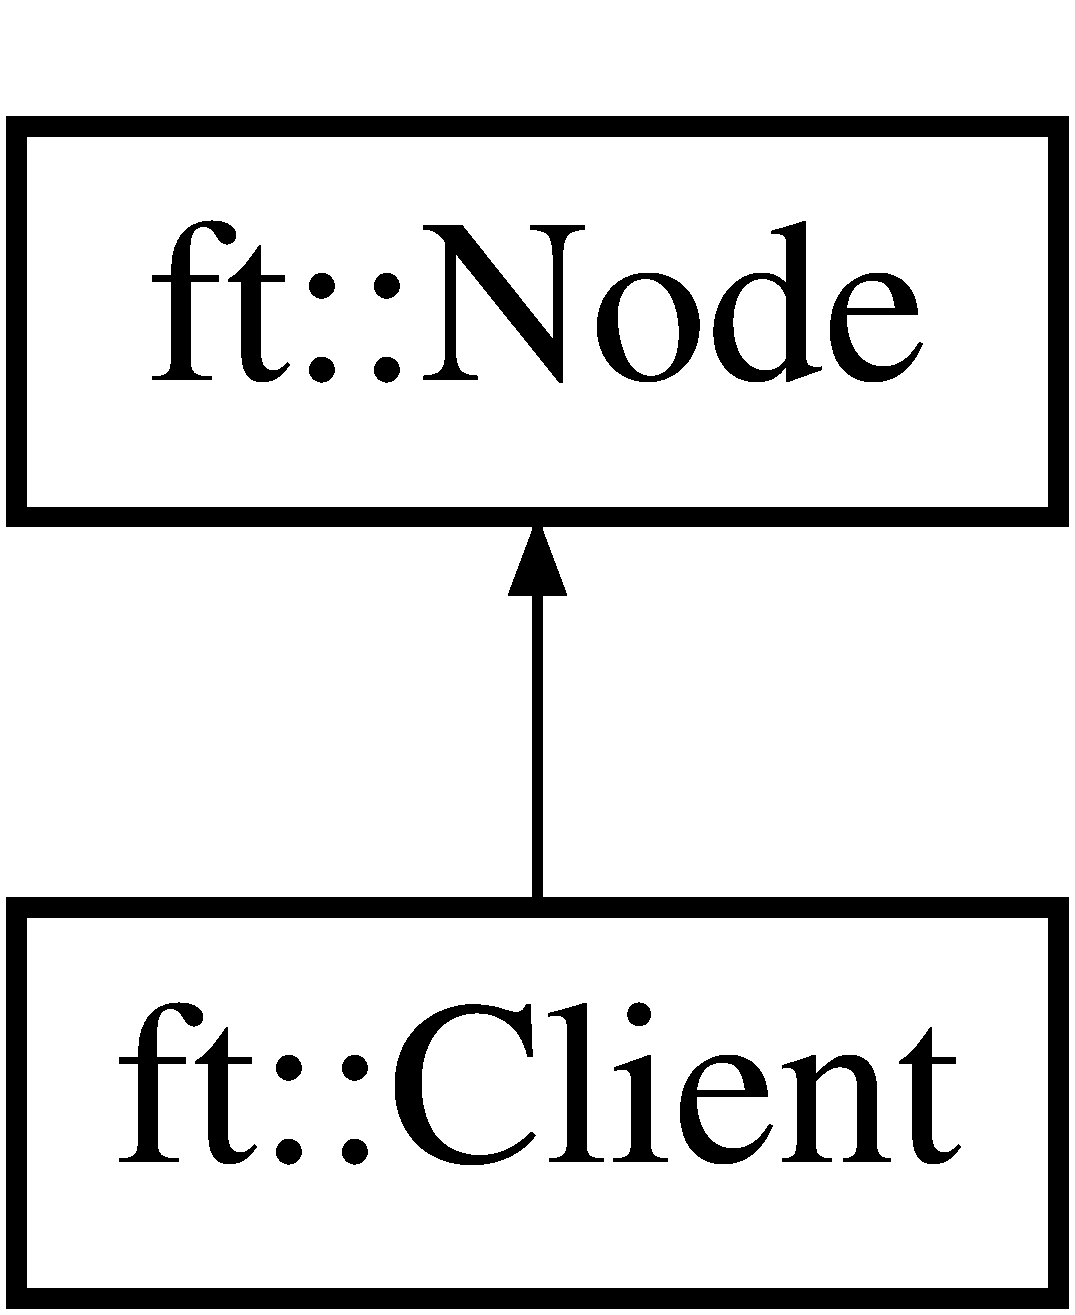
\includegraphics[height=2.000000cm]{classft_1_1Client}
\end{center}
\end{figure}
\subsection*{Public Member Functions}
\begin{DoxyCompactItemize}
\item 
int \mbox{\hyperlink{classft_1_1Client_a063db70469c9f2715bbad637d0353680}{initialize}} (std\+::string cfg\+\_\+file)
\item 
\mbox{\hyperlink{classft_1_1Shard}{ft\+::\+Shard}} $\ast$ \mbox{\hyperlink{classft_1_1Client_ac415215bb013b2d9832fe844c5d1c07a}{get\+Shard}} (unsigned long long key)
\item 
int \mbox{\hyperlink{classft_1_1Client_a345fef5f99ddffdd1c625bbceee918e0}{discover\+Primary}} (\mbox{\hyperlink{classft_1_1Shard}{ft\+::\+Shard}} $\ast$shard)
\end{DoxyCompactItemize}
\subsection*{Additional Inherited Members}


\subsection{Detailed Description}
\mbox{\hyperlink{classft_1_1Client}{Client}} \mbox{\hyperlink{classft_1_1Node}{Node}} definition 

\subsection{Member Function Documentation}
\mbox{\Hypertarget{classft_1_1Client_a345fef5f99ddffdd1c625bbceee918e0}\label{classft_1_1Client_a345fef5f99ddffdd1c625bbceee918e0}} 
\index{ft\+::\+Client@{ft\+::\+Client}!discover\+Primary@{discover\+Primary}}
\index{discover\+Primary@{discover\+Primary}!ft\+::\+Client@{ft\+::\+Client}}
\subsubsection{\texorpdfstring{discover\+Primary()}{discoverPrimary()}}
{\footnotesize\ttfamily int ft\+::\+Client\+::discover\+Primary (\begin{DoxyParamCaption}\item[{\mbox{\hyperlink{classft_1_1Shard}{ft\+::\+Shard}} $\ast$}]{shard }\end{DoxyParamCaption})}

Discover primary server for a shard


\begin{DoxyParams}{Parameters}
{\em shard} & -\/ pointer to \mbox{\hyperlink{classft_1_1Shard}{Shard}} to discover\\
\hline
\end{DoxyParams}
\begin{DoxyReturn}{Returns}
status. 0 on success, non-\/zero otherwise. 
\end{DoxyReturn}
\mbox{\Hypertarget{classft_1_1Client_ac415215bb013b2d9832fe844c5d1c07a}\label{classft_1_1Client_ac415215bb013b2d9832fe844c5d1c07a}} 
\index{ft\+::\+Client@{ft\+::\+Client}!get\+Shard@{get\+Shard}}
\index{get\+Shard@{get\+Shard}!ft\+::\+Client@{ft\+::\+Client}}
\subsubsection{\texorpdfstring{get\+Shard()}{getShard()}}
{\footnotesize\ttfamily \mbox{\hyperlink{classft_1_1Shard}{ft\+::\+Shard}}$\ast$ ft\+::\+Client\+::get\+Shard (\begin{DoxyParamCaption}\item[{unsigned long long}]{key }\end{DoxyParamCaption})}

Get the primary server storing a key


\begin{DoxyParams}{Parameters}
{\em key} & -\/ key whose primary server to search for\\
\hline
\end{DoxyParams}
\begin{DoxyReturn}{Returns}
\mbox{\hyperlink{classft_1_1Server}{Server}} storing key 
\end{DoxyReturn}
\mbox{\Hypertarget{classft_1_1Client_a063db70469c9f2715bbad637d0353680}\label{classft_1_1Client_a063db70469c9f2715bbad637d0353680}} 
\index{ft\+::\+Client@{ft\+::\+Client}!initialize@{initialize}}
\index{initialize@{initialize}!ft\+::\+Client@{ft\+::\+Client}}
\subsubsection{\texorpdfstring{initialize()}{initialize()}}
{\footnotesize\ttfamily int ft\+::\+Client\+::initialize (\begin{DoxyParamCaption}\item[{std\+::string}]{cfg\+\_\+file }\end{DoxyParamCaption})\hspace{0.3cm}{\ttfamily [virtual]}}

Initialize client

\begin{DoxyReturn}{Returns}
status. 0 on success, non-\/zero otherwise. 
\end{DoxyReturn}


Reimplemented from \mbox{\hyperlink{classft_1_1Node_addc92fd2c5cae12a8ea68c30b7202e91}{ft\+::\+Node}}.



The documentation for this class was generated from the following file\+:\begin{DoxyCompactItemize}
\item 
/root/cjdambro/grad-\/school/\+C\+S\+E498/gits/fault-\/tolerance/include/faulttolerance/client.\+h\end{DoxyCompactItemize}

\hypertarget{classKVCGConfig}{}\section{K\+V\+C\+G\+Config Class Reference}
\label{classKVCGConfig}\index{K\+V\+C\+G\+Config@{K\+V\+C\+G\+Config}}


{\ttfamily \#include $<$kvcg\+\_\+config.\+h$>$}

\subsection*{Public Member Functions}
\begin{DoxyCompactItemize}
\item 
int \mbox{\hyperlink{classKVCGConfig_a47206f279489aacccb9200f0bf9b36cf}{parse\+\_\+json\+\_\+file}} (std\+::string filename)
\item 
std\+::size\+\_\+t \mbox{\hyperlink{classKVCGConfig_a873ecf819a05b79ccced5e5dada7843f}{get\+\_\+checksum}} ()
\item 
std\+::vector$<$ \mbox{\hyperlink{classft_1_1Server}{ft\+::\+Server}} $\ast$ $>$ \mbox{\hyperlink{classKVCGConfig_a260449f62666e968566716e2ea2c47c2}{get\+Server\+List}} ()
\item 
cse498\+::\+Provider\+Type \mbox{\hyperlink{classKVCGConfig_a66862a874ddbbe54e7b696894b970539}{get\+Provider}} ()
\item 
int \mbox{\hyperlink{classKVCGConfig_a971fafd747cbe1c95f1253d80e5549c6}{get\+Server\+Port}} ()
\item 
int \mbox{\hyperlink{classKVCGConfig_a4c25599c2f79b6ad5acd5e03526864be}{get\+Client\+Port}} ()
\end{DoxyCompactItemize}


\subsection{Detailed Description}
Class to parse config file and store data 

\subsection{Member Function Documentation}
\mbox{\Hypertarget{classKVCGConfig_a873ecf819a05b79ccced5e5dada7843f}\label{classKVCGConfig_a873ecf819a05b79ccced5e5dada7843f}} 
\index{K\+V\+C\+G\+Config@{K\+V\+C\+G\+Config}!get\+\_\+checksum@{get\+\_\+checksum}}
\index{get\+\_\+checksum@{get\+\_\+checksum}!K\+V\+C\+G\+Config@{K\+V\+C\+G\+Config}}
\subsubsection{\texorpdfstring{get\+\_\+checksum()}{get\_checksum()}}
{\footnotesize\ttfamily std\+::size\+\_\+t K\+V\+C\+G\+Config\+::get\+\_\+checksum (\begin{DoxyParamCaption}{ }\end{DoxyParamCaption})}

Calculate and return a checksum for the configuration.

\begin{DoxyReturn}{Returns}
hash of config file 
\end{DoxyReturn}
\mbox{\Hypertarget{classKVCGConfig_a4c25599c2f79b6ad5acd5e03526864be}\label{classKVCGConfig_a4c25599c2f79b6ad5acd5e03526864be}} 
\index{K\+V\+C\+G\+Config@{K\+V\+C\+G\+Config}!get\+Client\+Port@{get\+Client\+Port}}
\index{get\+Client\+Port@{get\+Client\+Port}!K\+V\+C\+G\+Config@{K\+V\+C\+G\+Config}}
\subsubsection{\texorpdfstring{get\+Client\+Port()}{getClientPort()}}
{\footnotesize\ttfamily int K\+V\+C\+G\+Config\+::get\+Client\+Port (\begin{DoxyParamCaption}{ }\end{DoxyParamCaption})\hspace{0.3cm}{\ttfamily [inline]}}

Get the port for server-\/client communication

\begin{DoxyReturn}{Returns}
int for client port 
\end{DoxyReturn}
\mbox{\Hypertarget{classKVCGConfig_a66862a874ddbbe54e7b696894b970539}\label{classKVCGConfig_a66862a874ddbbe54e7b696894b970539}} 
\index{K\+V\+C\+G\+Config@{K\+V\+C\+G\+Config}!get\+Provider@{get\+Provider}}
\index{get\+Provider@{get\+Provider}!K\+V\+C\+G\+Config@{K\+V\+C\+G\+Config}}
\subsubsection{\texorpdfstring{get\+Provider()}{getProvider()}}
{\footnotesize\ttfamily cse498\+::\+Provider\+Type K\+V\+C\+G\+Config\+::get\+Provider (\begin{DoxyParamCaption}{ }\end{DoxyParamCaption})\hspace{0.3cm}{\ttfamily [inline]}}

Get the provider from config.

\begin{DoxyReturn}{Returns}
Provider\+Type for servers. 
\end{DoxyReturn}
\mbox{\Hypertarget{classKVCGConfig_a260449f62666e968566716e2ea2c47c2}\label{classKVCGConfig_a260449f62666e968566716e2ea2c47c2}} 
\index{K\+V\+C\+G\+Config@{K\+V\+C\+G\+Config}!get\+Server\+List@{get\+Server\+List}}
\index{get\+Server\+List@{get\+Server\+List}!K\+V\+C\+G\+Config@{K\+V\+C\+G\+Config}}
\subsubsection{\texorpdfstring{get\+Server\+List()}{getServerList()}}
{\footnotesize\ttfamily std\+::vector$<$\mbox{\hyperlink{classft_1_1Server}{ft\+::\+Server}}$\ast$$>$ K\+V\+C\+G\+Config\+::get\+Server\+List (\begin{DoxyParamCaption}{ }\end{DoxyParamCaption})\hspace{0.3cm}{\ttfamily [inline]}}

Get list of servers parsed from config.

\begin{DoxyReturn}{Returns}
vector of Servers 
\end{DoxyReturn}
\mbox{\Hypertarget{classKVCGConfig_a971fafd747cbe1c95f1253d80e5549c6}\label{classKVCGConfig_a971fafd747cbe1c95f1253d80e5549c6}} 
\index{K\+V\+C\+G\+Config@{K\+V\+C\+G\+Config}!get\+Server\+Port@{get\+Server\+Port}}
\index{get\+Server\+Port@{get\+Server\+Port}!K\+V\+C\+G\+Config@{K\+V\+C\+G\+Config}}
\subsubsection{\texorpdfstring{get\+Server\+Port()}{getServerPort()}}
{\footnotesize\ttfamily int K\+V\+C\+G\+Config\+::get\+Server\+Port (\begin{DoxyParamCaption}{ }\end{DoxyParamCaption})\hspace{0.3cm}{\ttfamily [inline]}}

Get the port for server-\/to-\/server communication

\begin{DoxyReturn}{Returns}
int for server port 
\end{DoxyReturn}
\mbox{\Hypertarget{classKVCGConfig_a47206f279489aacccb9200f0bf9b36cf}\label{classKVCGConfig_a47206f279489aacccb9200f0bf9b36cf}} 
\index{K\+V\+C\+G\+Config@{K\+V\+C\+G\+Config}!parse\+\_\+json\+\_\+file@{parse\+\_\+json\+\_\+file}}
\index{parse\+\_\+json\+\_\+file@{parse\+\_\+json\+\_\+file}!K\+V\+C\+G\+Config@{K\+V\+C\+G\+Config}}
\subsubsection{\texorpdfstring{parse\+\_\+json\+\_\+file()}{parse\_json\_file()}}
{\footnotesize\ttfamily int K\+V\+C\+G\+Config\+::parse\+\_\+json\+\_\+file (\begin{DoxyParamCaption}\item[{std\+::string}]{filename }\end{DoxyParamCaption})}

Parse J\+S\+ON input file


\begin{DoxyParams}{Parameters}
{\em filename} & -\/ name of J\+S\+ON file to parse\\
\hline
\end{DoxyParams}
\begin{DoxyReturn}{Returns}
status. 0 on success, non-\/zero otherwise. 
\end{DoxyReturn}


The documentation for this class was generated from the following file\+:\begin{DoxyCompactItemize}
\item 
/root/cjdambro/grad-\/school/\+C\+S\+E498/gits/fault-\/tolerance/include/faulttolerance/kvcg\+\_\+config.\+h\end{DoxyCompactItemize}

\hypertarget{classft_1_1Node}{}\section{ft\+:\+:Node Class Reference}
\label{classft_1_1Node}\index{ft\+::\+Node@{ft\+::\+Node}}


{\ttfamily \#include $<$node.\+h$>$}

Inheritance diagram for ft\+:\+:Node\+:\begin{figure}[H]
\begin{center}
\leavevmode
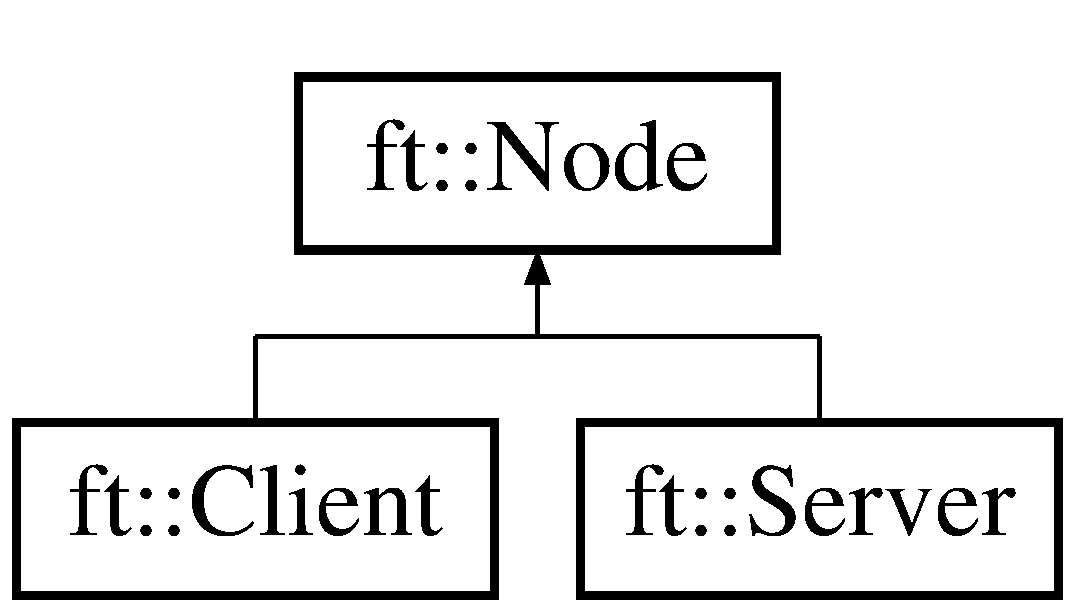
\includegraphics[height=2.000000cm]{classft_1_1Node}
\end{center}
\end{figure}
\subsection*{Public Member Functions}
\begin{DoxyCompactItemize}
\item 
virtual int \mbox{\hyperlink{classft_1_1Node_addc92fd2c5cae12a8ea68c30b7202e91}{initialize}} (std\+::string cfg\+\_\+file)
\item 
void \mbox{\hyperlink{classft_1_1Node_a0a09f86d4b043b0da034e7da0d83463c}{set\+Name}} (std\+::string n)
\item 
void \mbox{\hyperlink{classft_1_1Node_af2fde6292b45c9a7e85a8905c8c728cc}{set\+Addr}} (std\+::string a)
\item 
std\+::string \mbox{\hyperlink{classft_1_1Node_af62312cc4d5a05c859034b10b1a1af64}{get\+Name}} ()
\item 
std\+::string \mbox{\hyperlink{classft_1_1Node_aabbf4a7cd8fcea779622b65a4bf75e94}{get\+Addr}} ()
\item 
int \mbox{\hyperlink{classft_1_1Node_ad936b7c83c1169f04fe5c73ccca2a99d}{get\+Client\+Port}} ()
\item 
cse498\+::\+Provider\+Type \mbox{\hyperlink{classft_1_1Node_ae6115aceb38ad07ba4afd6fa7cd7f9aa}{get\+Provider}} ()
\item 
\mbox{\Hypertarget{classft_1_1Node_a01c39aea51e51007be97a4a18c05d938}\label{classft_1_1Node_a01c39aea51e51007be97a4a18c05d938}} 
bool {\bfseries operator$<$} (const \mbox{\hyperlink{classft_1_1Node}{ft\+::\+Node}} \&o) const
\end{DoxyCompactItemize}
\subsection*{Public Attributes}
\begin{DoxyCompactItemize}
\item 
\mbox{\Hypertarget{classft_1_1Node_aecc8e36018ee507399fdc5e3f561a500}\label{classft_1_1Node_aecc8e36018ee507399fdc5e3f561a500}} 
bool {\bfseries alive} = true
\end{DoxyCompactItemize}
\subsection*{Protected Attributes}
\begin{DoxyCompactItemize}
\item 
\mbox{\Hypertarget{classft_1_1Node_a46124887e675ddcd5bfdba6c4a015964}\label{classft_1_1Node_a46124887e675ddcd5bfdba6c4a015964}} 
std\+::string {\bfseries hostname}
\item 
\mbox{\Hypertarget{classft_1_1Node_ac321a30ddc190fe5a3ec93869adaf82d}\label{classft_1_1Node_ac321a30ddc190fe5a3ec93869adaf82d}} 
std\+::string {\bfseries addr} = \char`\"{}\char`\"{}
\item 
\mbox{\Hypertarget{classft_1_1Node_a520e4c96f13e8ce7cea0c8bf21b83c5f}\label{classft_1_1Node_a520e4c96f13e8ce7cea0c8bf21b83c5f}} 
int {\bfseries client\+Port}
\item 
\mbox{\Hypertarget{classft_1_1Node_a3f16f19902a912ce42a81439b6f4500e}\label{classft_1_1Node_a3f16f19902a912ce42a81439b6f4500e}} 
cse498\+::\+Provider\+Type {\bfseries provider}
\item 
\mbox{\Hypertarget{classft_1_1Node_ab4561d8c56968bfe211550eeea205761}\label{classft_1_1Node_ab4561d8c56968bfe211550eeea205761}} 
size\+\_\+t {\bfseries cksum}
\end{DoxyCompactItemize}


\subsection{Detailed Description}
Base class for \mbox{\hyperlink{classft_1_1Server}{Server}} and \mbox{\hyperlink{classft_1_1Client}{Client}} 

\subsection{Member Function Documentation}
\mbox{\Hypertarget{classft_1_1Node_aabbf4a7cd8fcea779622b65a4bf75e94}\label{classft_1_1Node_aabbf4a7cd8fcea779622b65a4bf75e94}} 
\index{ft\+::\+Node@{ft\+::\+Node}!get\+Addr@{get\+Addr}}
\index{get\+Addr@{get\+Addr}!ft\+::\+Node@{ft\+::\+Node}}
\subsubsection{\texorpdfstring{get\+Addr()}{getAddr()}}
{\footnotesize\ttfamily std\+::string ft\+::\+Node\+::get\+Addr (\begin{DoxyParamCaption}{ }\end{DoxyParamCaption})\hspace{0.3cm}{\ttfamily [inline]}}

Get the address of the node

\begin{DoxyReturn}{Returns}
Addres of node 
\end{DoxyReturn}
\mbox{\Hypertarget{classft_1_1Node_ad936b7c83c1169f04fe5c73ccca2a99d}\label{classft_1_1Node_ad936b7c83c1169f04fe5c73ccca2a99d}} 
\index{ft\+::\+Node@{ft\+::\+Node}!get\+Client\+Port@{get\+Client\+Port}}
\index{get\+Client\+Port@{get\+Client\+Port}!ft\+::\+Node@{ft\+::\+Node}}
\subsubsection{\texorpdfstring{get\+Client\+Port()}{getClientPort()}}
{\footnotesize\ttfamily int ft\+::\+Node\+::get\+Client\+Port (\begin{DoxyParamCaption}{ }\end{DoxyParamCaption})\hspace{0.3cm}{\ttfamily [inline]}}

Get the client port of the node

\begin{DoxyReturn}{Returns}
The client port of node 
\end{DoxyReturn}
\mbox{\Hypertarget{classft_1_1Node_af62312cc4d5a05c859034b10b1a1af64}\label{classft_1_1Node_af62312cc4d5a05c859034b10b1a1af64}} 
\index{ft\+::\+Node@{ft\+::\+Node}!get\+Name@{get\+Name}}
\index{get\+Name@{get\+Name}!ft\+::\+Node@{ft\+::\+Node}}
\subsubsection{\texorpdfstring{get\+Name()}{getName()}}
{\footnotesize\ttfamily std\+::string ft\+::\+Node\+::get\+Name (\begin{DoxyParamCaption}{ }\end{DoxyParamCaption})\hspace{0.3cm}{\ttfamily [inline]}}

Get the name of the node

\begin{DoxyReturn}{Returns}
Name of the node 
\end{DoxyReturn}
\mbox{\Hypertarget{classft_1_1Node_ae6115aceb38ad07ba4afd6fa7cd7f9aa}\label{classft_1_1Node_ae6115aceb38ad07ba4afd6fa7cd7f9aa}} 
\index{ft\+::\+Node@{ft\+::\+Node}!get\+Provider@{get\+Provider}}
\index{get\+Provider@{get\+Provider}!ft\+::\+Node@{ft\+::\+Node}}
\subsubsection{\texorpdfstring{get\+Provider()}{getProvider()}}
{\footnotesize\ttfamily cse498\+::\+Provider\+Type ft\+::\+Node\+::get\+Provider (\begin{DoxyParamCaption}{ }\end{DoxyParamCaption})\hspace{0.3cm}{\ttfamily [inline]}}

Get the provider of the node

\begin{DoxyReturn}{Returns}
The provider of node 
\end{DoxyReturn}
\mbox{\Hypertarget{classft_1_1Node_addc92fd2c5cae12a8ea68c30b7202e91}\label{classft_1_1Node_addc92fd2c5cae12a8ea68c30b7202e91}} 
\index{ft\+::\+Node@{ft\+::\+Node}!initialize@{initialize}}
\index{initialize@{initialize}!ft\+::\+Node@{ft\+::\+Node}}
\subsubsection{\texorpdfstring{initialize()}{initialize()}}
{\footnotesize\ttfamily virtual int ft\+::\+Node\+::initialize (\begin{DoxyParamCaption}\item[{std\+::string}]{cfg\+\_\+file }\end{DoxyParamCaption})\hspace{0.3cm}{\ttfamily [inline]}, {\ttfamily [virtual]}}

Initialize node data 

Reimplemented in \mbox{\hyperlink{classft_1_1Server_a834002a833999b593d357b72ef69ddcf}{ft\+::\+Server}}, and \mbox{\hyperlink{classft_1_1Client_a063db70469c9f2715bbad637d0353680}{ft\+::\+Client}}.

\mbox{\Hypertarget{classft_1_1Node_af2fde6292b45c9a7e85a8905c8c728cc}\label{classft_1_1Node_af2fde6292b45c9a7e85a8905c8c728cc}} 
\index{ft\+::\+Node@{ft\+::\+Node}!set\+Addr@{set\+Addr}}
\index{set\+Addr@{set\+Addr}!ft\+::\+Node@{ft\+::\+Node}}
\subsubsection{\texorpdfstring{set\+Addr()}{setAddr()}}
{\footnotesize\ttfamily void ft\+::\+Node\+::set\+Addr (\begin{DoxyParamCaption}\item[{std\+::string}]{a }\end{DoxyParamCaption})\hspace{0.3cm}{\ttfamily [inline]}}

Set the address of the node


\begin{DoxyParams}{Parameters}
{\em a} & -\/ Address to set for node \\
\hline
\end{DoxyParams}
\mbox{\Hypertarget{classft_1_1Node_a0a09f86d4b043b0da034e7da0d83463c}\label{classft_1_1Node_a0a09f86d4b043b0da034e7da0d83463c}} 
\index{ft\+::\+Node@{ft\+::\+Node}!set\+Name@{set\+Name}}
\index{set\+Name@{set\+Name}!ft\+::\+Node@{ft\+::\+Node}}
\subsubsection{\texorpdfstring{set\+Name()}{setName()}}
{\footnotesize\ttfamily void ft\+::\+Node\+::set\+Name (\begin{DoxyParamCaption}\item[{std\+::string}]{n }\end{DoxyParamCaption})\hspace{0.3cm}{\ttfamily [inline]}}

Set the name of the node


\begin{DoxyParams}{Parameters}
{\em n} & -\/ Name to set for node \\
\hline
\end{DoxyParams}


The documentation for this class was generated from the following file\+:\begin{DoxyCompactItemize}
\item 
/root/cjdambro/grad-\/school/\+C\+S\+E498/gits/fault-\/tolerance/include/faulttolerance/node.\+h\end{DoxyCompactItemize}

\hypertarget{classft_1_1Server}{}\section{ft\+:\+:Server Class Reference}
\label{classft_1_1Server}\index{ft\+::\+Server@{ft\+::\+Server}}


{\ttfamily \#include $<$server.\+h$>$}

Inheritance diagram for ft\+:\+:Server\+:\begin{figure}[H]
\begin{center}
\leavevmode
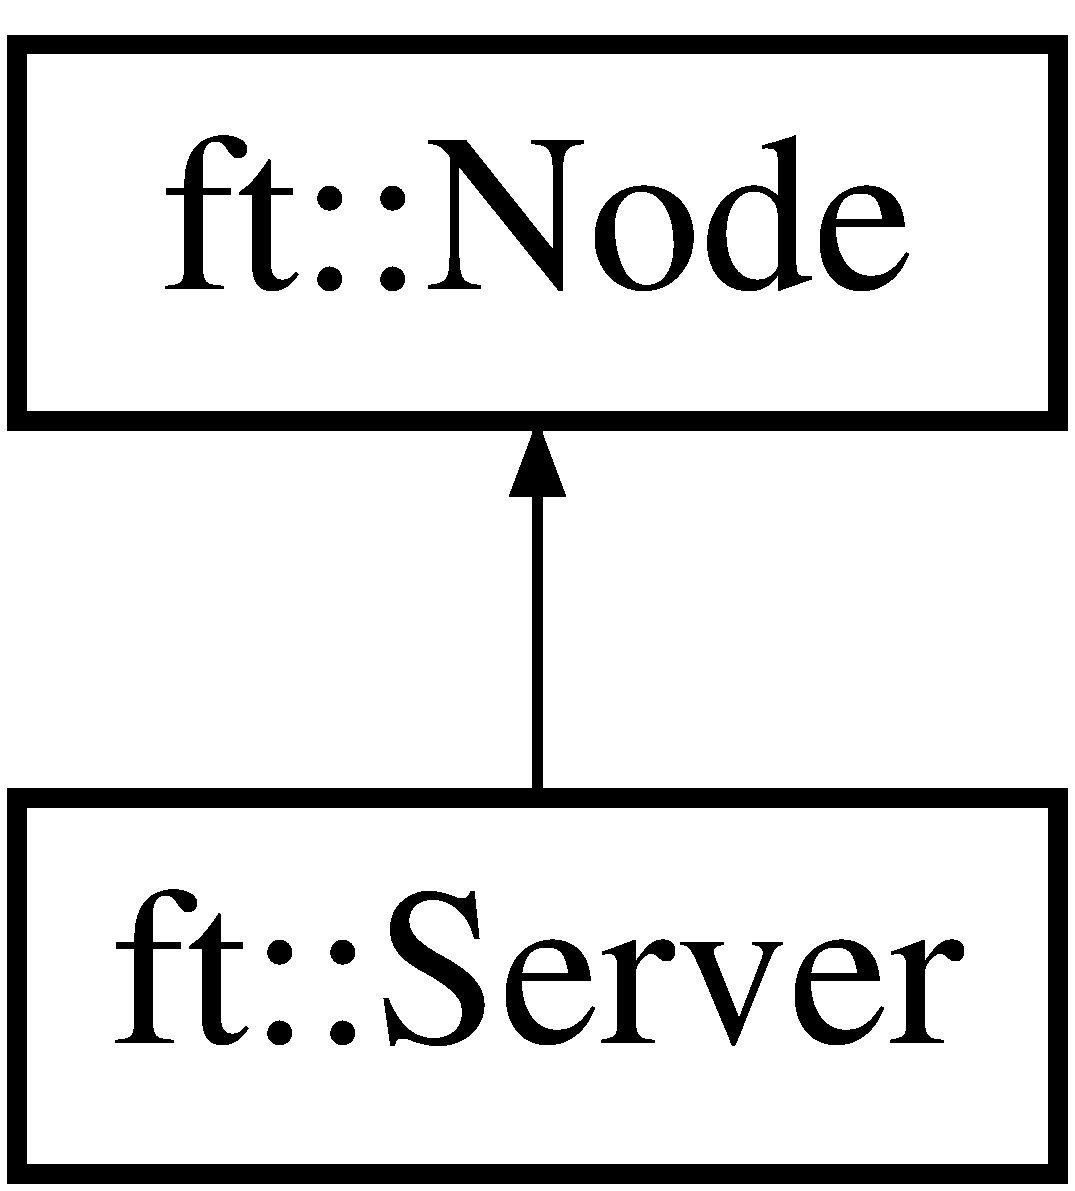
\includegraphics[height=2.000000cm]{classft_1_1Server}
\end{center}
\end{figure}
\subsection*{Public Member Functions}
\begin{DoxyCompactItemize}
\item 
\mbox{\Hypertarget{classft_1_1Server_a63475cd47ee0ffbbbb323059f83cbd27}\label{classft_1_1Server_a63475cd47ee0ffbbbb323059f83cbd27}} 
\mbox{\hyperlink{classft_1_1Server}{Server}} \& {\bfseries operator=} (const \mbox{\hyperlink{classft_1_1Server}{ft\+::\+Server}} \&\&src)
\item 
int \mbox{\hyperlink{classft_1_1Server_a834002a833999b593d357b72ef69ddcf}{initialize}} (std\+::string cfg\+\_\+file)
\item 
void \mbox{\hyperlink{classft_1_1Server_a4df01ccbcc6295e4930e3c65dedaa595}{shutdown\+Server}} ()
\item 
void \mbox{\hyperlink{classft_1_1Server_a0c333cc78d88ff7ada32ffff429a8788}{print\+Server}} (const Log\+Level lvl)
\item 
std\+::vector$<$ std\+::pair$<$ unsigned long long, unsigned long long $>$ $>$ \mbox{\hyperlink{classft_1_1Server_a86cc643b14f616c8ba0ecaddbbb696eb}{get\+Primary\+Keys}} ()
\item 
bool \mbox{\hyperlink{classft_1_1Server_a5f5dd98bd5956bb480f4e8564c7620cd}{add\+Key\+Range}} (std\+::pair$<$ unsigned long long, unsigned long long $>$ key\+Range)
\item 
bool \mbox{\hyperlink{classft_1_1Server_a395dbe95b7c78b48213a62b4bc2d7c9d}{add\+Primary\+Server}} (\mbox{\hyperlink{classft_1_1Server}{ft\+::\+Server}} $\ast$s)
\item 
std\+::vector$<$ \mbox{\hyperlink{classft_1_1Server}{ft\+::\+Server}} $\ast$ $>$ \mbox{\hyperlink{classft_1_1Server_a97e94c9e9c8ed5eb8282564f1d2db739}{get\+Backup\+Servers}} ()
\item 
bool \mbox{\hyperlink{classft_1_1Server_a2458eef12718b2f04129a68ddea466c3}{add\+Backup\+Server}} (\mbox{\hyperlink{classft_1_1Server}{ft\+::\+Server}} $\ast$s)
\item 
bool \mbox{\hyperlink{classft_1_1Server_ac3c476b8dad7bbb3fb39470c79dc2a6e}{is\+Primary}} (unsigned long long key)
\item 
bool \mbox{\hyperlink{classft_1_1Server_aae86da697b404a1337b94b2a1ee7d5ed}{is\+Backup}} (unsigned long long key)
\item 
int \mbox{\hyperlink{classft_1_1Server_a17e80f813ff788007ece482e5d311ffa}{log\+Request}} (unsigned long long key, data\+\_\+t $\ast$value)
\item 
int \mbox{\hyperlink{classft_1_1Server_ae97719e0790afb356374955130cb4c72}{log\+Request}} (std\+::vector$<$ unsigned long long $>$ keys, std\+::vector$<$ data\+\_\+t $\ast$$>$ values)
\item 
int \mbox{\hyperlink{classft_1_1Server_ada92c4dbf92ee02bb99be77a9faae1e2}{log\+Request}} (std\+::vector$<$ Request\+Wrapper$<$ unsigned long long, data\+\_\+t $\ast$$>$$>$ batch)
\item 
std\+::size\+\_\+t \mbox{\hyperlink{classft_1_1Server_aef123896c2f84d6bc2c5fe2940d1a8b4}{get\+Hash}} ()
\end{DoxyCompactItemize}
\subsection*{Public Attributes}
\begin{DoxyCompactItemize}
\item 
\mbox{\Hypertarget{classft_1_1Server_abd5204ed28334489e0358975cd3e9f34}\label{classft_1_1Server_abd5204ed28334489e0358975cd3e9f34}} 
cse498\+::\+Connection $\ast$ {\bfseries primary\+\_\+conn}
\item 
\mbox{\Hypertarget{classft_1_1Server_ac99b52438e80a92645fcc6b6c57e2f6b}\label{classft_1_1Server_ac99b52438e80a92645fcc6b6c57e2f6b}} 
cse498\+::\+Connection $\ast$ {\bfseries backup\+\_\+conn}
\end{DoxyCompactItemize}
\subsection*{Additional Inherited Members}


\subsection{Detailed Description}
\mbox{\hyperlink{classft_1_1Server}{Server}} \mbox{\hyperlink{classft_1_1Node}{Node}} definition 

\subsection{Member Function Documentation}
\mbox{\Hypertarget{classft_1_1Server_a2458eef12718b2f04129a68ddea466c3}\label{classft_1_1Server_a2458eef12718b2f04129a68ddea466c3}} 
\index{ft\+::\+Server@{ft\+::\+Server}!add\+Backup\+Server@{add\+Backup\+Server}}
\index{add\+Backup\+Server@{add\+Backup\+Server}!ft\+::\+Server@{ft\+::\+Server}}
\subsubsection{\texorpdfstring{add\+Backup\+Server()}{addBackupServer()}}
{\footnotesize\ttfamily bool ft\+::\+Server\+::add\+Backup\+Server (\begin{DoxyParamCaption}\item[{\mbox{\hyperlink{classft_1_1Server}{ft\+::\+Server}} $\ast$}]{s }\end{DoxyParamCaption})}

Add server who is backing this one up


\begin{DoxyParams}{Parameters}
{\em s} & -\/ \mbox{\hyperlink{classft_1_1Server}{Server}} to add to backup server list\\
\hline
\end{DoxyParams}
\begin{DoxyReturn}{Returns}
true if added successfully, false otherwise 
\end{DoxyReturn}
\mbox{\Hypertarget{classft_1_1Server_a5f5dd98bd5956bb480f4e8564c7620cd}\label{classft_1_1Server_a5f5dd98bd5956bb480f4e8564c7620cd}} 
\index{ft\+::\+Server@{ft\+::\+Server}!add\+Key\+Range@{add\+Key\+Range}}
\index{add\+Key\+Range@{add\+Key\+Range}!ft\+::\+Server@{ft\+::\+Server}}
\subsubsection{\texorpdfstring{add\+Key\+Range()}{addKeyRange()}}
{\footnotesize\ttfamily bool ft\+::\+Server\+::add\+Key\+Range (\begin{DoxyParamCaption}\item[{std\+::pair$<$ unsigned long long, unsigned long long $>$}]{key\+Range }\end{DoxyParamCaption})}

Add key range to primary list


\begin{DoxyParams}{Parameters}
{\em key\+Range} & -\/ pair of min and max key\\
\hline
\end{DoxyParams}
\begin{DoxyReturn}{Returns}
true if added successfully, false otherwise 
\end{DoxyReturn}
\mbox{\Hypertarget{classft_1_1Server_a395dbe95b7c78b48213a62b4bc2d7c9d}\label{classft_1_1Server_a395dbe95b7c78b48213a62b4bc2d7c9d}} 
\index{ft\+::\+Server@{ft\+::\+Server}!add\+Primary\+Server@{add\+Primary\+Server}}
\index{add\+Primary\+Server@{add\+Primary\+Server}!ft\+::\+Server@{ft\+::\+Server}}
\subsubsection{\texorpdfstring{add\+Primary\+Server()}{addPrimaryServer()}}
{\footnotesize\ttfamily bool ft\+::\+Server\+::add\+Primary\+Server (\begin{DoxyParamCaption}\item[{\mbox{\hyperlink{classft_1_1Server}{ft\+::\+Server}} $\ast$}]{s }\end{DoxyParamCaption})}

Add server who this one is backing up


\begin{DoxyParams}{Parameters}
{\em s} & -\/ \mbox{\hyperlink{classft_1_1Server}{Server}} to add to primary server list\\
\hline
\end{DoxyParams}
\begin{DoxyReturn}{Returns}
true if added successfully, false otherwise 
\end{DoxyReturn}
\mbox{\Hypertarget{classft_1_1Server_a97e94c9e9c8ed5eb8282564f1d2db739}\label{classft_1_1Server_a97e94c9e9c8ed5eb8282564f1d2db739}} 
\index{ft\+::\+Server@{ft\+::\+Server}!get\+Backup\+Servers@{get\+Backup\+Servers}}
\index{get\+Backup\+Servers@{get\+Backup\+Servers}!ft\+::\+Server@{ft\+::\+Server}}
\subsubsection{\texorpdfstring{get\+Backup\+Servers()}{getBackupServers()}}
{\footnotesize\ttfamily std\+::vector$<$\mbox{\hyperlink{classft_1_1Server}{ft\+::\+Server}}$\ast$$>$ ft\+::\+Server\+::get\+Backup\+Servers (\begin{DoxyParamCaption}{ }\end{DoxyParamCaption})\hspace{0.3cm}{\ttfamily [inline]}}

Get list of servers acting as this one\textquotesingle{}s backup

\begin{DoxyReturn}{Returns}
vector of backup servers 
\end{DoxyReturn}
\mbox{\Hypertarget{classft_1_1Server_aef123896c2f84d6bc2c5fe2940d1a8b4}\label{classft_1_1Server_aef123896c2f84d6bc2c5fe2940d1a8b4}} 
\index{ft\+::\+Server@{ft\+::\+Server}!get\+Hash@{get\+Hash}}
\index{get\+Hash@{get\+Hash}!ft\+::\+Server@{ft\+::\+Server}}
\subsubsection{\texorpdfstring{get\+Hash()}{getHash()}}
{\footnotesize\ttfamily std\+::size\+\_\+t ft\+::\+Server\+::get\+Hash (\begin{DoxyParamCaption}{ }\end{DoxyParamCaption})}

Get a hash value of this server configuration

\begin{DoxyReturn}{Returns}
hash of the server 
\end{DoxyReturn}
\mbox{\Hypertarget{classft_1_1Server_a86cc643b14f616c8ba0ecaddbbb696eb}\label{classft_1_1Server_a86cc643b14f616c8ba0ecaddbbb696eb}} 
\index{ft\+::\+Server@{ft\+::\+Server}!get\+Primary\+Keys@{get\+Primary\+Keys}}
\index{get\+Primary\+Keys@{get\+Primary\+Keys}!ft\+::\+Server@{ft\+::\+Server}}
\subsubsection{\texorpdfstring{get\+Primary\+Keys()}{getPrimaryKeys()}}
{\footnotesize\ttfamily std\+::vector$<$std\+::pair$<$unsigned long long, unsigned long long$>$ $>$ ft\+::\+Server\+::get\+Primary\+Keys (\begin{DoxyParamCaption}{ }\end{DoxyParamCaption})\hspace{0.3cm}{\ttfamily [inline]}}

Get vector of primary key ranges

\begin{DoxyReturn}{Returns}
vector of min/max key range pairs 
\end{DoxyReturn}
\mbox{\Hypertarget{classft_1_1Server_a834002a833999b593d357b72ef69ddcf}\label{classft_1_1Server_a834002a833999b593d357b72ef69ddcf}} 
\index{ft\+::\+Server@{ft\+::\+Server}!initialize@{initialize}}
\index{initialize@{initialize}!ft\+::\+Server@{ft\+::\+Server}}
\subsubsection{\texorpdfstring{initialize()}{initialize()}}
{\footnotesize\ttfamily int ft\+::\+Server\+::initialize (\begin{DoxyParamCaption}\item[{std\+::string}]{cfg\+\_\+file }\end{DoxyParamCaption})\hspace{0.3cm}{\ttfamily [virtual]}}

Initialize server

\begin{DoxyReturn}{Returns}
status. 0 on success, non-\/zero otherwise. 
\end{DoxyReturn}


Reimplemented from \mbox{\hyperlink{classft_1_1Node_addc92fd2c5cae12a8ea68c30b7202e91}{ft\+::\+Node}}.

\mbox{\Hypertarget{classft_1_1Server_aae86da697b404a1337b94b2a1ee7d5ed}\label{classft_1_1Server_aae86da697b404a1337b94b2a1ee7d5ed}} 
\index{ft\+::\+Server@{ft\+::\+Server}!is\+Backup@{is\+Backup}}
\index{is\+Backup@{is\+Backup}!ft\+::\+Server@{ft\+::\+Server}}
\subsubsection{\texorpdfstring{is\+Backup()}{isBackup()}}
{\footnotesize\ttfamily bool ft\+::\+Server\+::is\+Backup (\begin{DoxyParamCaption}\item[{unsigned long long}]{key }\end{DoxyParamCaption})}

Check if server is backing up a given key


\begin{DoxyParams}{Parameters}
{\em key} & -\/ key to check if backing up\\
\hline
\end{DoxyParams}
\begin{DoxyReturn}{Returns}
true if backing, false otherwise 
\end{DoxyReturn}
\mbox{\Hypertarget{classft_1_1Server_ac3c476b8dad7bbb3fb39470c79dc2a6e}\label{classft_1_1Server_ac3c476b8dad7bbb3fb39470c79dc2a6e}} 
\index{ft\+::\+Server@{ft\+::\+Server}!is\+Primary@{is\+Primary}}
\index{is\+Primary@{is\+Primary}!ft\+::\+Server@{ft\+::\+Server}}
\subsubsection{\texorpdfstring{is\+Primary()}{isPrimary()}}
{\footnotesize\ttfamily bool ft\+::\+Server\+::is\+Primary (\begin{DoxyParamCaption}\item[{unsigned long long}]{key }\end{DoxyParamCaption})}

Check if server is running as primary for a given key


\begin{DoxyParams}{Parameters}
{\em key} & -\/ key to check if primary\\
\hline
\end{DoxyParams}
\begin{DoxyReturn}{Returns}
true if primary, false otherwise 
\end{DoxyReturn}
\mbox{\Hypertarget{classft_1_1Server_a17e80f813ff788007ece482e5d311ffa}\label{classft_1_1Server_a17e80f813ff788007ece482e5d311ffa}} 
\index{ft\+::\+Server@{ft\+::\+Server}!log\+Request@{log\+Request}}
\index{log\+Request@{log\+Request}!ft\+::\+Server@{ft\+::\+Server}}
\subsubsection{\texorpdfstring{log\+Request()}{logRequest()}\hspace{0.1cm}{\footnotesize\ttfamily [1/3]}}
{\footnotesize\ttfamily int ft\+::\+Server\+::log\+Request (\begin{DoxyParamCaption}\item[{unsigned long long}]{key,  }\item[{data\+\_\+t $\ast$}]{value }\end{DoxyParamCaption})}

Log a P\+UT transaction to all backup servers.


\begin{DoxyParams}{Parameters}
{\em key} & -\/ value of key in table \\
\hline
{\em value} & -\/ data to store in table at key\\
\hline
\end{DoxyParams}
\begin{DoxyReturn}{Returns}
0 on success, non-\/zero on failure 
\end{DoxyReturn}
\mbox{\Hypertarget{classft_1_1Server_ae97719e0790afb356374955130cb4c72}\label{classft_1_1Server_ae97719e0790afb356374955130cb4c72}} 
\index{ft\+::\+Server@{ft\+::\+Server}!log\+Request@{log\+Request}}
\index{log\+Request@{log\+Request}!ft\+::\+Server@{ft\+::\+Server}}
\subsubsection{\texorpdfstring{log\+Request()}{logRequest()}\hspace{0.1cm}{\footnotesize\ttfamily [2/3]}}
{\footnotesize\ttfamily int ft\+::\+Server\+::log\+Request (\begin{DoxyParamCaption}\item[{std\+::vector$<$ unsigned long long $>$}]{keys,  }\item[{std\+::vector$<$ data\+\_\+t $\ast$$>$}]{values }\end{DoxyParamCaption})}

Log a batch of P\+UT transactions to backup servers.


\begin{DoxyParams}{Parameters}
{\em keys} & -\/ vector of keys to update \\
\hline
{\em values} & -\/ vector of data to store at keys\\
\hline
\end{DoxyParams}
\begin{DoxyReturn}{Returns}
0 on success, non-\/zero on failure 
\end{DoxyReturn}
\mbox{\Hypertarget{classft_1_1Server_ada92c4dbf92ee02bb99be77a9faae1e2}\label{classft_1_1Server_ada92c4dbf92ee02bb99be77a9faae1e2}} 
\index{ft\+::\+Server@{ft\+::\+Server}!log\+Request@{log\+Request}}
\index{log\+Request@{log\+Request}!ft\+::\+Server@{ft\+::\+Server}}
\subsubsection{\texorpdfstring{log\+Request()}{logRequest()}\hspace{0.1cm}{\footnotesize\ttfamily [3/3]}}
{\footnotesize\ttfamily int ft\+::\+Server\+::log\+Request (\begin{DoxyParamCaption}\item[{std\+::vector$<$ Request\+Wrapper$<$ unsigned long long, data\+\_\+t $\ast$$>$$>$}]{batch }\end{DoxyParamCaption})}

Log a batch of Request\+Wrapper transactions to backup servers.


\begin{DoxyParams}{Parameters}
{\em batch} & -\/ batch of backup requests\\
\hline
\end{DoxyParams}
\begin{DoxyReturn}{Returns}
0 on success, non-\/zero on failure 
\end{DoxyReturn}
\mbox{\Hypertarget{classft_1_1Server_a0c333cc78d88ff7ada32ffff429a8788}\label{classft_1_1Server_a0c333cc78d88ff7ada32ffff429a8788}} 
\index{ft\+::\+Server@{ft\+::\+Server}!print\+Server@{print\+Server}}
\index{print\+Server@{print\+Server}!ft\+::\+Server@{ft\+::\+Server}}
\subsubsection{\texorpdfstring{print\+Server()}{printServer()}}
{\footnotesize\ttfamily void ft\+::\+Server\+::print\+Server (\begin{DoxyParamCaption}\item[{const Log\+Level}]{lvl }\end{DoxyParamCaption})}

Print server configuration if log level $>$ lvl


\begin{DoxyParams}{Parameters}
{\em lvl} & -\/ log level to start printing. Will print more at higher levels. \\
\hline
\end{DoxyParams}
\mbox{\Hypertarget{classft_1_1Server_a4df01ccbcc6295e4930e3c65dedaa595}\label{classft_1_1Server_a4df01ccbcc6295e4930e3c65dedaa595}} 
\index{ft\+::\+Server@{ft\+::\+Server}!shutdown\+Server@{shutdown\+Server}}
\index{shutdown\+Server@{shutdown\+Server}!ft\+::\+Server@{ft\+::\+Server}}
\subsubsection{\texorpdfstring{shutdown\+Server()}{shutdownServer()}}
{\footnotesize\ttfamily void ft\+::\+Server\+::shutdown\+Server (\begin{DoxyParamCaption}{ }\end{DoxyParamCaption})}

Shutdown server 

The documentation for this class was generated from the following file\+:\begin{DoxyCompactItemize}
\item 
/root/cjdambro/grad-\/school/\+C\+S\+E498/gits/fault-\/tolerance/include/faulttolerance/server.\+h\end{DoxyCompactItemize}

\hypertarget{classft_1_1Shard}{}\section{ft\+:\+:Shard Class Reference}
\label{classft_1_1Shard}\index{ft\+::\+Shard@{ft\+::\+Shard}}
\subsection*{Public Member Functions}
\begin{DoxyCompactItemize}
\item 
\mbox{\Hypertarget{classft_1_1Shard_a12f4f5734184d8c7382cbbe66d1d26ed}\label{classft_1_1Shard_a12f4f5734184d8c7382cbbe66d1d26ed}} 
{\bfseries Shard} (std\+::pair$<$ unsigned long long, unsigned long long $>$ kr)
\item 
void \mbox{\hyperlink{classft_1_1Shard_a2d393309209fc78d93ccf0bb3426c431}{add\+Server}} (\mbox{\hyperlink{classft_1_1Server}{ft\+::\+Server}} $\ast$s)
\item 
\mbox{\hyperlink{classft_1_1Server}{ft\+::\+Server}} $\ast$ \mbox{\hyperlink{classft_1_1Shard_a76b726de0fb962f51f453c68ebe751e3}{get\+Primary}} ()
\item 
void \mbox{\hyperlink{classft_1_1Shard_a9a850b8347f8be6b939f00ee91463da7}{set\+Primary}} (\mbox{\hyperlink{classft_1_1Server}{ft\+::\+Server}} $\ast$s)
\item 
int \mbox{\hyperlink{classft_1_1Shard_accde84c93a127987f75dccc9c57275b5}{discover\+Primary}} ()
\item 
bool \mbox{\hyperlink{classft_1_1Shard_a42e25665d6fc9d6075d0477e3470c293}{contains\+Key}} (unsigned long long key)
\item 
unsigned long long \mbox{\hyperlink{classft_1_1Shard_a5c75dfb7d06ed5ff8a1ceeca7b199576}{get\+Lower\+Bound}} ()
\item 
unsigned long long \mbox{\hyperlink{classft_1_1Shard_adf483639946d24a658d2e07a498e08b2}{get\+Upper\+Bound}} ()
\item 
std\+::vector$<$ \mbox{\hyperlink{classft_1_1Server}{ft\+::\+Server}} $\ast$ $>$ \mbox{\hyperlink{classft_1_1Shard_ac06fd0bca4f4254d114401ecb58d744f}{get\+Servers}} ()
\end{DoxyCompactItemize}


\subsection{Member Function Documentation}
\mbox{\Hypertarget{classft_1_1Shard_a2d393309209fc78d93ccf0bb3426c431}\label{classft_1_1Shard_a2d393309209fc78d93ccf0bb3426c431}} 
\index{ft\+::\+Shard@{ft\+::\+Shard}!add\+Server@{add\+Server}}
\index{add\+Server@{add\+Server}!ft\+::\+Shard@{ft\+::\+Shard}}
\subsubsection{\texorpdfstring{add\+Server()}{addServer()}}
{\footnotesize\ttfamily void ft\+::\+Shard\+::add\+Server (\begin{DoxyParamCaption}\item[{\mbox{\hyperlink{classft_1_1Server}{ft\+::\+Server}} $\ast$}]{s }\end{DoxyParamCaption})\hspace{0.3cm}{\ttfamily [inline]}}

Add a server to this \mbox{\hyperlink{classft_1_1Shard}{Shard}}


\begin{DoxyParams}{Parameters}
{\em s} & -\/ server to add \\
\hline
\end{DoxyParams}
\mbox{\Hypertarget{classft_1_1Shard_a42e25665d6fc9d6075d0477e3470c293}\label{classft_1_1Shard_a42e25665d6fc9d6075d0477e3470c293}} 
\index{ft\+::\+Shard@{ft\+::\+Shard}!contains\+Key@{contains\+Key}}
\index{contains\+Key@{contains\+Key}!ft\+::\+Shard@{ft\+::\+Shard}}
\subsubsection{\texorpdfstring{contains\+Key()}{containsKey()}}
{\footnotesize\ttfamily bool ft\+::\+Shard\+::contains\+Key (\begin{DoxyParamCaption}\item[{unsigned long long}]{key }\end{DoxyParamCaption})\hspace{0.3cm}{\ttfamily [inline]}}

Determine if this \mbox{\hyperlink{classft_1_1Shard}{Shard}} contains a given key


\begin{DoxyParams}{Parameters}
{\em key} & -\/ key to check in \mbox{\hyperlink{classft_1_1Shard}{Shard}}\\
\hline
\end{DoxyParams}
\begin{DoxyReturn}{Returns}
true if contains key, false otherwise 
\end{DoxyReturn}
\mbox{\Hypertarget{classft_1_1Shard_accde84c93a127987f75dccc9c57275b5}\label{classft_1_1Shard_accde84c93a127987f75dccc9c57275b5}} 
\index{ft\+::\+Shard@{ft\+::\+Shard}!discover\+Primary@{discover\+Primary}}
\index{discover\+Primary@{discover\+Primary}!ft\+::\+Shard@{ft\+::\+Shard}}
\subsubsection{\texorpdfstring{discover\+Primary()}{discoverPrimary()}}
{\footnotesize\ttfamily int ft\+::\+Shard\+::discover\+Primary (\begin{DoxyParamCaption}{ }\end{DoxyParamCaption})}

Discover primary server for a shard to be cached in that shard

\begin{DoxyReturn}{Returns}
status. 0 on success, non-\/zero otherwise. 
\end{DoxyReturn}
\mbox{\Hypertarget{classft_1_1Shard_a5c75dfb7d06ed5ff8a1ceeca7b199576}\label{classft_1_1Shard_a5c75dfb7d06ed5ff8a1ceeca7b199576}} 
\index{ft\+::\+Shard@{ft\+::\+Shard}!get\+Lower\+Bound@{get\+Lower\+Bound}}
\index{get\+Lower\+Bound@{get\+Lower\+Bound}!ft\+::\+Shard@{ft\+::\+Shard}}
\subsubsection{\texorpdfstring{get\+Lower\+Bound()}{getLowerBound()}}
{\footnotesize\ttfamily unsigned long long ft\+::\+Shard\+::get\+Lower\+Bound (\begin{DoxyParamCaption}{ }\end{DoxyParamCaption})\hspace{0.3cm}{\ttfamily [inline]}}

Get the lower bound on this \mbox{\hyperlink{classft_1_1Shard}{Shard}}\textquotesingle{}s key range

\begin{DoxyReturn}{Returns}
lower key value 
\end{DoxyReturn}
\mbox{\Hypertarget{classft_1_1Shard_a76b726de0fb962f51f453c68ebe751e3}\label{classft_1_1Shard_a76b726de0fb962f51f453c68ebe751e3}} 
\index{ft\+::\+Shard@{ft\+::\+Shard}!get\+Primary@{get\+Primary}}
\index{get\+Primary@{get\+Primary}!ft\+::\+Shard@{ft\+::\+Shard}}
\subsubsection{\texorpdfstring{get\+Primary()}{getPrimary()}}
{\footnotesize\ttfamily \mbox{\hyperlink{classft_1_1Server}{ft\+::\+Server}}$\ast$ ft\+::\+Shard\+::get\+Primary (\begin{DoxyParamCaption}{ }\end{DoxyParamCaption})\hspace{0.3cm}{\ttfamily [inline]}}

Get the cached primary for this \mbox{\hyperlink{classft_1_1Shard}{Shard}}

\begin{DoxyReturn}{Returns}
current primary server 
\end{DoxyReturn}
\mbox{\Hypertarget{classft_1_1Shard_ac06fd0bca4f4254d114401ecb58d744f}\label{classft_1_1Shard_ac06fd0bca4f4254d114401ecb58d744f}} 
\index{ft\+::\+Shard@{ft\+::\+Shard}!get\+Servers@{get\+Servers}}
\index{get\+Servers@{get\+Servers}!ft\+::\+Shard@{ft\+::\+Shard}}
\subsubsection{\texorpdfstring{get\+Servers()}{getServers()}}
{\footnotesize\ttfamily std\+::vector$<$\mbox{\hyperlink{classft_1_1Server}{ft\+::\+Server}}$\ast$$>$ ft\+::\+Shard\+::get\+Servers (\begin{DoxyParamCaption}{ }\end{DoxyParamCaption})\hspace{0.3cm}{\ttfamily [inline]}}

Get the list of servers in this \mbox{\hyperlink{classft_1_1Shard}{Shard}}

\begin{DoxyReturn}{Returns}
list of servers 
\end{DoxyReturn}
\mbox{\Hypertarget{classft_1_1Shard_adf483639946d24a658d2e07a498e08b2}\label{classft_1_1Shard_adf483639946d24a658d2e07a498e08b2}} 
\index{ft\+::\+Shard@{ft\+::\+Shard}!get\+Upper\+Bound@{get\+Upper\+Bound}}
\index{get\+Upper\+Bound@{get\+Upper\+Bound}!ft\+::\+Shard@{ft\+::\+Shard}}
\subsubsection{\texorpdfstring{get\+Upper\+Bound()}{getUpperBound()}}
{\footnotesize\ttfamily unsigned long long ft\+::\+Shard\+::get\+Upper\+Bound (\begin{DoxyParamCaption}{ }\end{DoxyParamCaption})\hspace{0.3cm}{\ttfamily [inline]}}

Get the upper bound on this \mbox{\hyperlink{classft_1_1Shard}{Shard}}\textquotesingle{}s key range

\begin{DoxyReturn}{Returns}
upper key value 
\end{DoxyReturn}
\mbox{\Hypertarget{classft_1_1Shard_a9a850b8347f8be6b939f00ee91463da7}\label{classft_1_1Shard_a9a850b8347f8be6b939f00ee91463da7}} 
\index{ft\+::\+Shard@{ft\+::\+Shard}!set\+Primary@{set\+Primary}}
\index{set\+Primary@{set\+Primary}!ft\+::\+Shard@{ft\+::\+Shard}}
\subsubsection{\texorpdfstring{set\+Primary()}{setPrimary()}}
{\footnotesize\ttfamily void ft\+::\+Shard\+::set\+Primary (\begin{DoxyParamCaption}\item[{\mbox{\hyperlink{classft_1_1Server}{ft\+::\+Server}} $\ast$}]{s }\end{DoxyParamCaption})\hspace{0.3cm}{\ttfamily [inline]}}

Set the current primary in this \mbox{\hyperlink{classft_1_1Shard}{Shard}}\textquotesingle{}s cached data


\begin{DoxyParams}{Parameters}
{\em s} & -\/ \mbox{\hyperlink{classft_1_1Server}{Server}} pointer to primary \\
\hline
\end{DoxyParams}


The documentation for this class was generated from the following file\+:\begin{DoxyCompactItemize}
\item 
/root/cjdambro/grad-\/school/\+C\+S\+E498/gits/fault-\/tolerance/include/faulttolerance/shard.\+h\end{DoxyCompactItemize}

\chapter{File Documentation}
\hypertarget{fault__tolerance_8h}{}\section{/root/cjdambro/grad-\/school/\+C\+S\+E498/gits/fault-\/tolerance/include/faulttolerance/fault\+\_\+tolerance.h File Reference}
\label{fault__tolerance_8h}\index{/root/cjdambro/grad-\/school/\+C\+S\+E498/gits/fault-\/tolerance/include/faulttolerance/fault\+\_\+tolerance.\+h@{/root/cjdambro/grad-\/school/\+C\+S\+E498/gits/fault-\/tolerance/include/faulttolerance/fault\+\_\+tolerance.\+h}}


Public A\+PI for K\+V\+CG Fault Tolerance protocol.  


{\ttfamily \#include $<$faulttolerance/node.\+h$>$}\newline
{\ttfamily \#include $<$faulttolerance/server.\+h$>$}\newline
{\ttfamily \#include $<$faulttolerance/client.\+h$>$}\newline


\subsection{Detailed Description}
Public A\+PI for K\+V\+CG Fault Tolerance protocol. 


%--- End generated contents ---

% Index
\backmatter
\newpage
\phantomsection
\clearemptydoublepage
\addcontentsline{toc}{chapter}{Index}
\printindex

\end{document}
